% Print results for comparing MSN with 2D Runge function

\begin{figure}[p]
    \centering
    \begin{subfigure}{0.45\textwidth}
    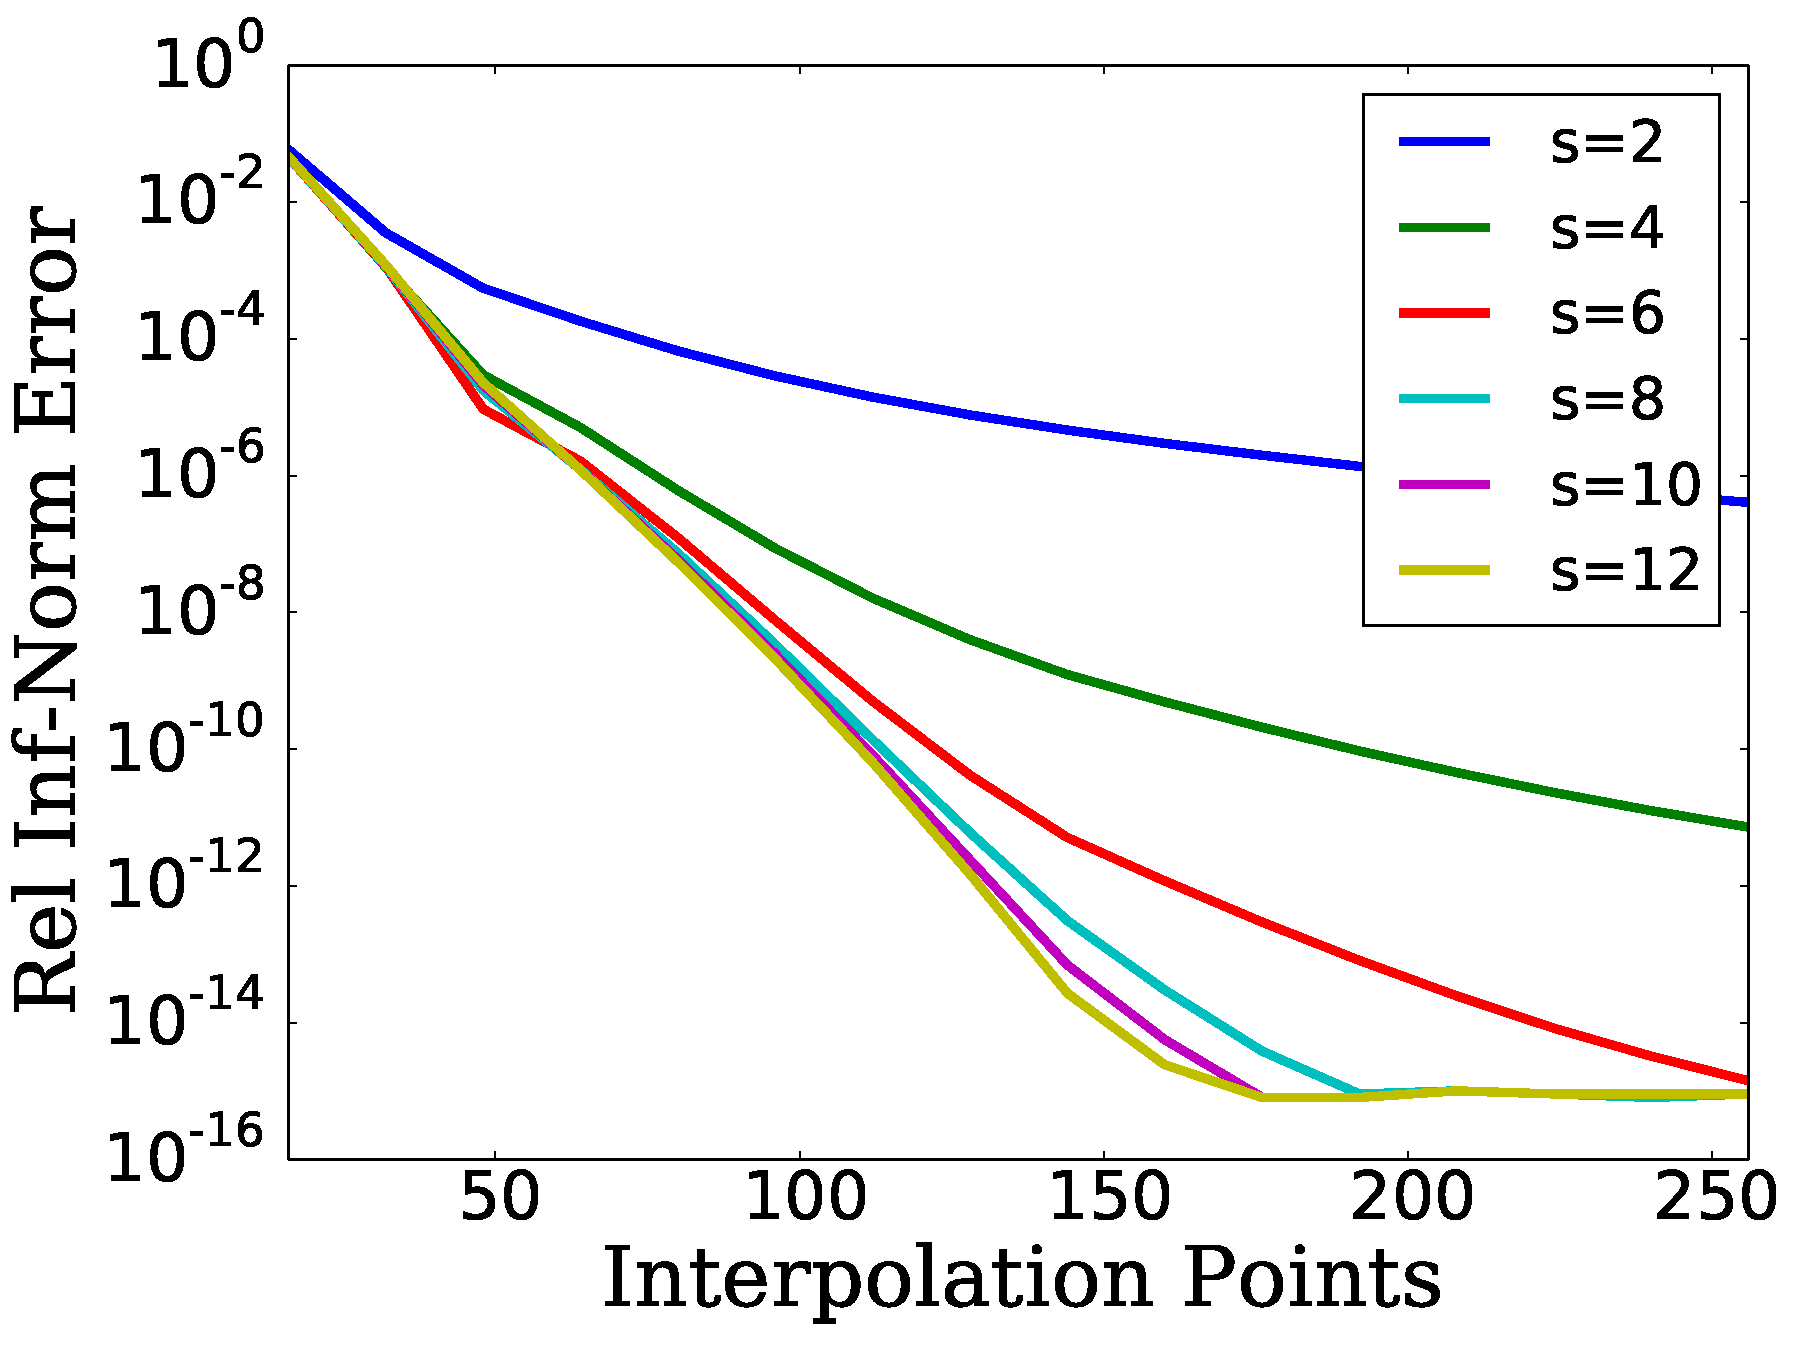
\includegraphics[width=\textwidth]{plots/msn_1d_smooth_R_25.pdf}
    \caption{$R=25$}
    \end{subfigure}
    \begin{subfigure}{0.45\textwidth}
    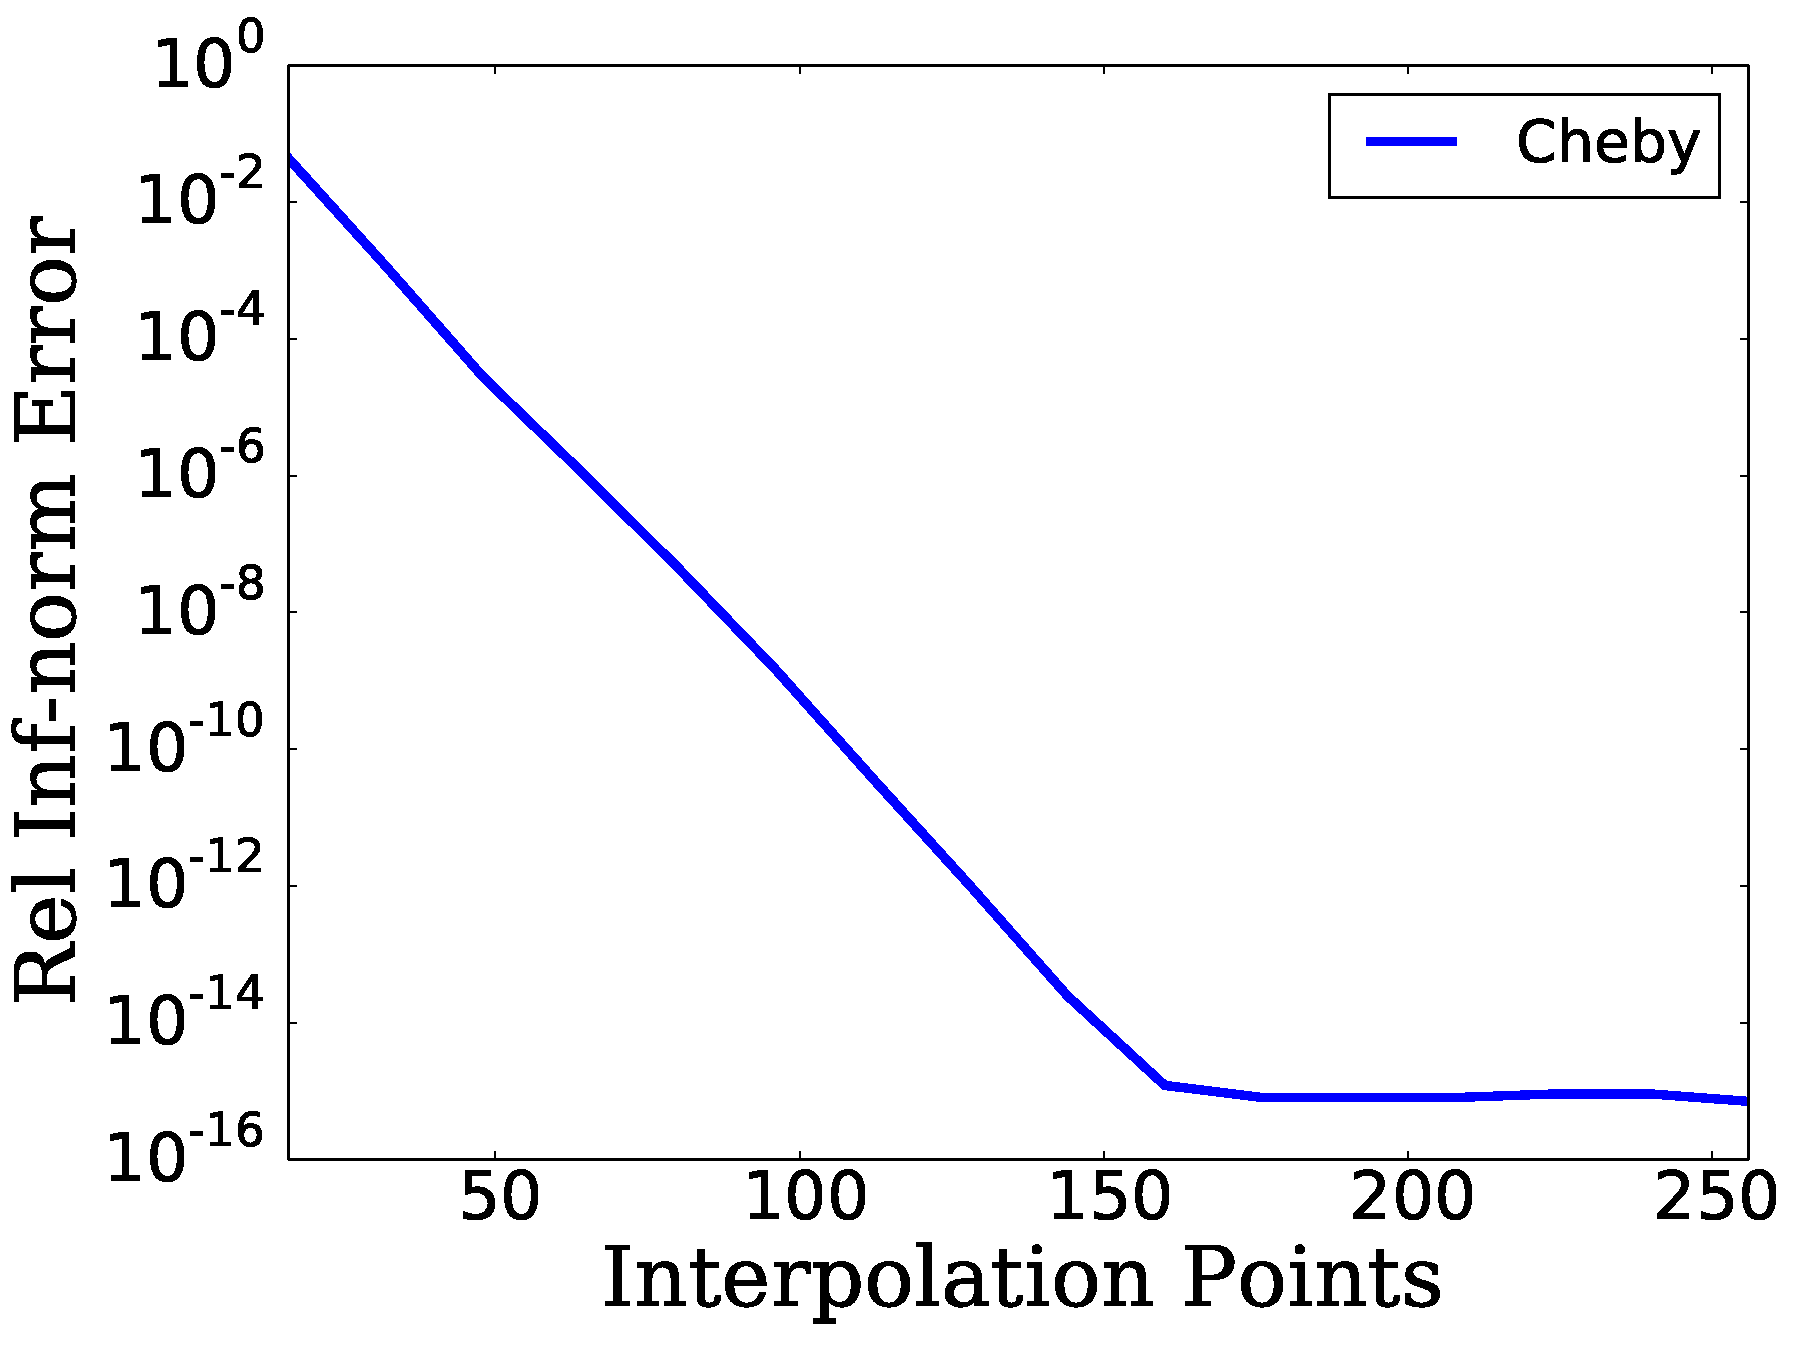
\includegraphics[width=\textwidth]{plots/cheby_1d_smooth_R_25.pdf}
    \caption{$R=25$}
    \end{subfigure}

    \begin{subfigure}{0.45\textwidth}
    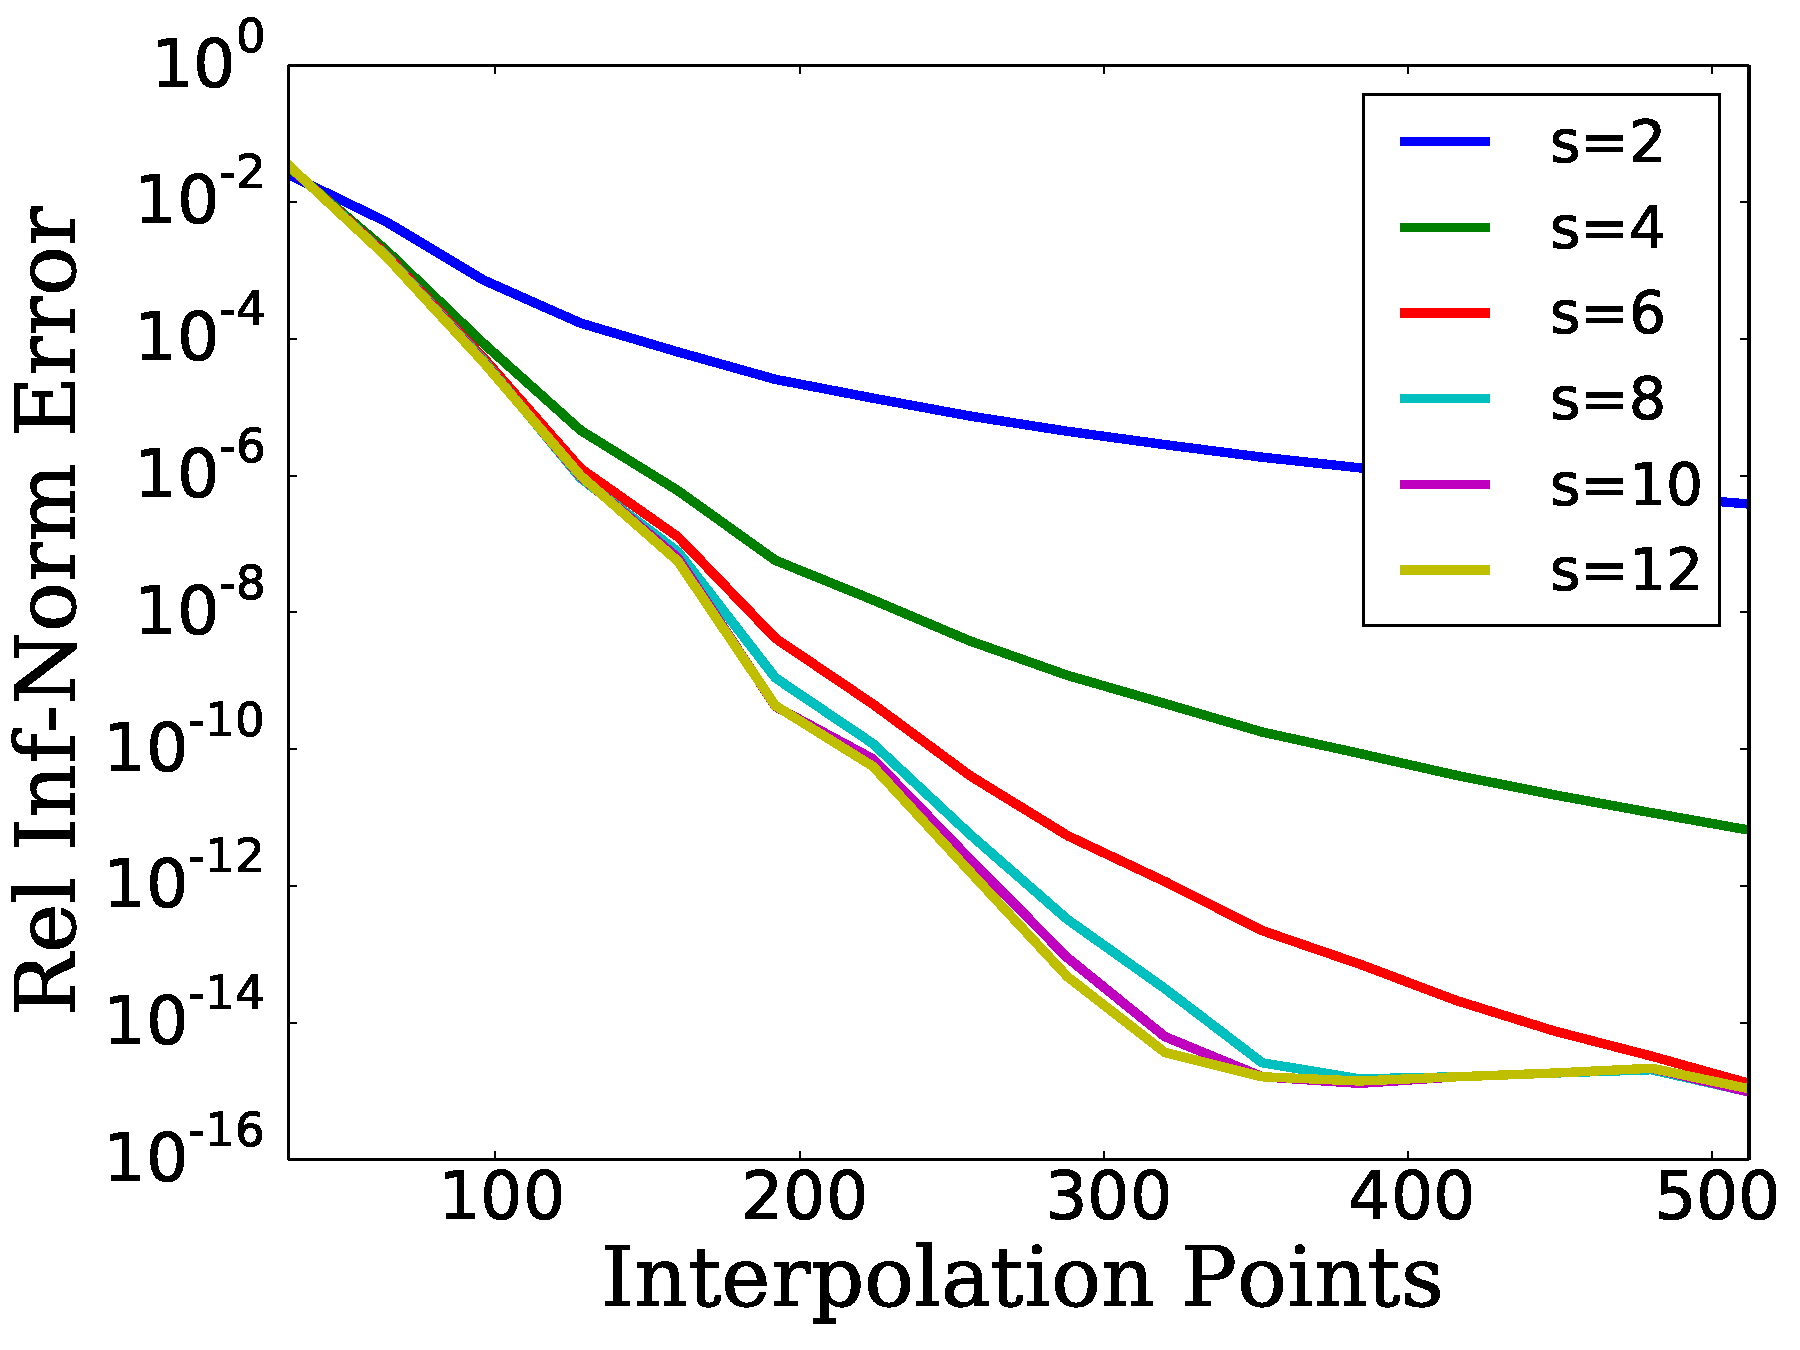
\includegraphics[width=\textwidth]{plots/msn_1d_smooth_R_100.pdf}
    \caption{$R=100$}
    \end{subfigure}
    \begin{subfigure}{0.45\textwidth}
    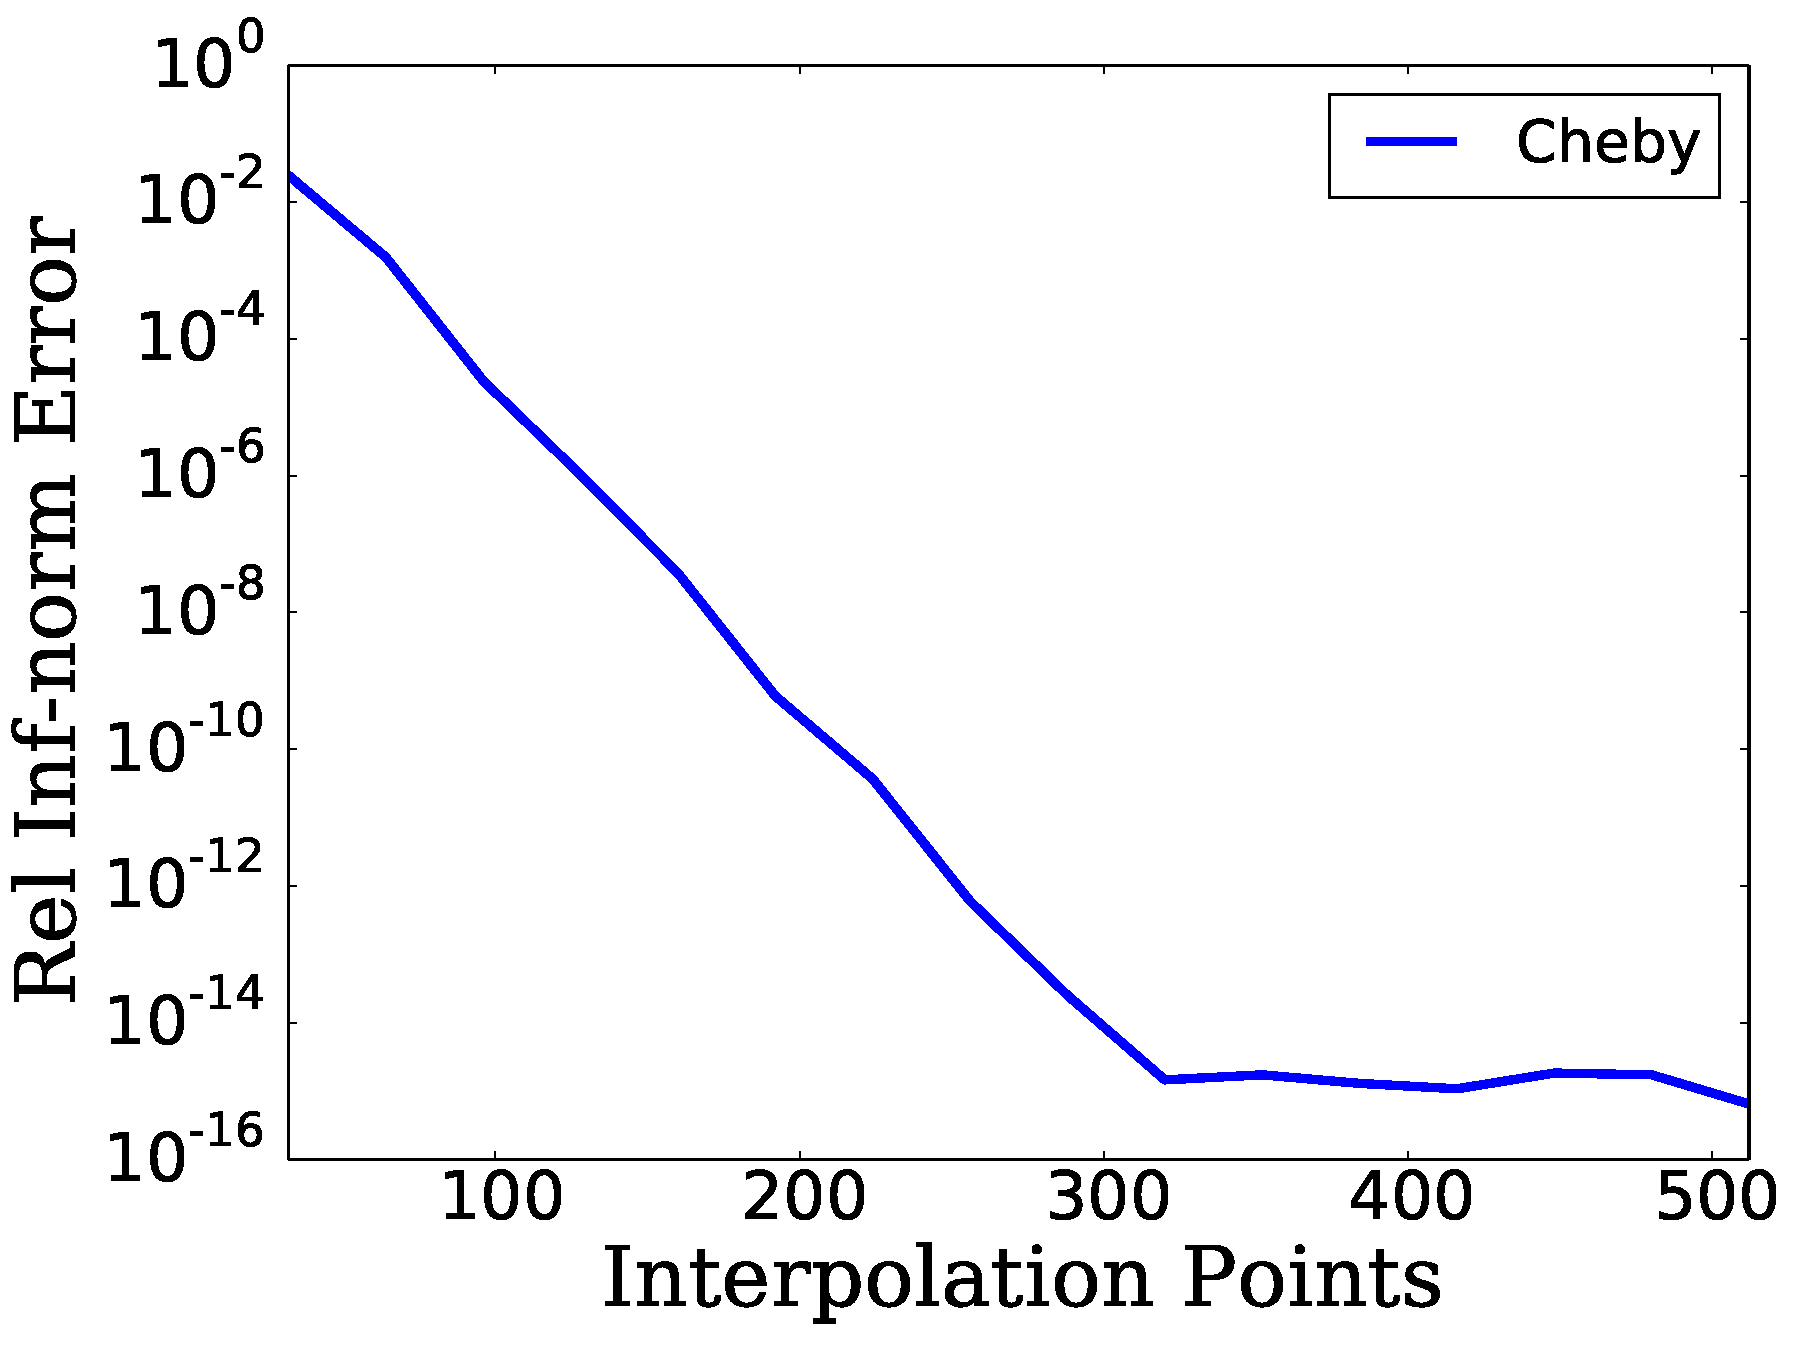
\includegraphics[width=\textwidth]{plots/cheby_1d_smooth_R_100.pdf}
    \caption{$R=100$}
    \end{subfigure}

\caption[Smooth Interpolation Comparison: 1D Runge Function]{
MSN interpolation and Chebyshev interpolation results of the
1D Runge function $g_{25}$ and $g_{100}$ for various $s$ values.
}
\label{fig:smooth_comparison_1d_runge}
\end{figure}



